%Version 3.1 December 2024 (Springer Nature LaTeX template, sn-jnl class)
% Phase 4 research paper -- CS3001 Computer Networks, FAST-NUCES Islamabad
% Compile with pdfLaTeX + BibTeX (Overleaf default). Figures are in figures/.
\documentclass[pdflatex,iicol,sn-mathphys-num]{sn-jnl}

\usepackage{graphicx}%
\usepackage{multirow}%
\usepackage{amsmath,amssymb,amsfonts}%
\usepackage{amsthm}%
\usepackage{mathrsfs}%
\usepackage[title]{appendix}%
\usepackage{xcolor}%
\usepackage{textcomp}%
\usepackage{manyfoot}%
\usepackage{booktabs}%
\usepackage{algorithm}%
\usepackage{algorithmicx}%
\usepackage{algpseudocode}%
\usepackage{listings}%
\usepackage{array}%
\usepackage{tabularx}%
\newcolumntype{Y}{>{\raggedright\arraybackslash}X}%

\newcommand{\yes}{\checkmark}
\newcommand{\no}{--}

\raggedbottom

\begin{document}

\title[Fidelity and Cost of XAI for Encrypted-Traffic IDS]{Evaluating the Fidelity and Computational Cost of Explainable AI for Encrypted Network Traffic Intrusion Detection}

\author*[1]{\fnm{Ahmed} \sur{Raza}}\email{i240026@isb.nu.edu.pk}

\author[1]{\fnm{Huzaifa} \sur{Mudassar}}\email{i240050@isb.nu.edu.pk}

\affil*[1]{\orgdiv{Department of Artificial Intelligence and Data Science}, \orgname{National University of Computer and Emerging Sciences (FAST-NUCES)}, \orgaddress{\city{Islamabad}, \country{Pakistan}}}

\abstract{Most network traffic is now encrypted, so an intrusion detection system (IDS) sees only flow metadata such as packet sizes, timing and direction. Explainable AI (XAI) methods such as SHAP and LIME help analysts trust its alerts, but their per-flow cost and their correctness on metadata-only features are rarely measured, and no work decides which flows to explain under a real-time budget. This paper measures the cost, faithfulness and cross-network consistency of nine explainers on five detectors under plaintext-, TLS~1.3- and QUIC-level visibility on CIC-IDS2017, CSE-CIC-IDS2018 and HIKARI-2021, and proposes a budget-aware selective explanation trigger. Model-specific explainers such as TreeSHAP cost about as much as detection (about 1\,ms per flow), while KernelSHAP and LIME need 7--524\,ms, up to 1{,}500 times more, and the most faithful explainer is model-specific in 8 of 10 dataset--detector pairs. Hiding ports and TCP headers raised faithfulness for 7 of 8 pairs on CIC-IDS2017, and explanation drift across networks followed the loss in recall (Spearman $\rho_s=0.63$). During a port-scan flood, the trigger explained every alert within 1\,s at an overhead of 0.105 of detection time and a 35\,ms delay, 74.9\% and 98.7\% below explaining every alert. Choosing the explainer with the detector and explaining selectively therefore make per-alert explanation practical for encrypted-traffic IDS.}

\keywords{Explainable AI, Intrusion detection, Encrypted traffic, SHAP, Explanation cost, Selective explanation}

\maketitle

%% ================================================================
\section{Introduction}\label{sec:intro}

Most network traffic is now encrypted. TLS~1.3 hides the payload and most handshake fields~\cite{rfc8446}, and QUIC also encrypts the transport header~\cite{rfc9000}. An intrusion detection system (IDS) on such traffic can only use flow metadata: packet sizes, inter-arrival times, directions and volumes. An alert without a reason is hard for an analyst to trust, so explainers such as SHAP~\cite{lundberg2017,lundberg2020} and LIME~\cite{ribeiro2016} are increasingly attached to IDS alerts.

Four gaps remain. First, \emph{what does an explanation cost?} An IDS must keep up with line rate, but perturbation explainers call the model hundreds of times per flow. Existing work explains offline~\cite{kalakoti2026}, skips per-flow explanation~\cite{dmthreatnet2026} or times only classification~\cite{cerasuolo2026} (gap G1). Second, \emph{are explanations correct when only metadata is visible?} Fidelity metrics exist~\cite{bhatt2020,samek2017,yeh2019}, but they have been applied to plaintext-era features such as ports and TCP flags~\cite{p2,p6,p10}, which encryption removes (G2). Third, \emph{do explanations change when the network changes?} Detection accuracy collapses on a new network~\cite{cerasuolo2026,p9}, but the explanations have not been compared (G3). Finally, no work decides \emph{which} flows to explain within a fixed compute budget (G4).

This paper answers four research questions, each with a hypothesis from Phase~2: the time and memory each explainer adds (RQ1; H1: perturbation explainers slow each flow at least 100 times); how fidelity changes when only QUIC-level metadata is visible (RQ2; H2: fidelity and explainer agreement fall); whether explanations of the same attack agree across networks (RQ3; H3: agreement is lower across than within networks, and its drop follows the loss in accuracy); and whether a budget-aware trigger can explain alerts in time at low cost (RQ4; H4: overhead $\le$0.10 of detection time, $\ge$95\% of true alerts explained within 1\,s, no loss of fidelity). The contributions are:
\begin{itemize}
\item A joint measurement of the cost and fidelity of nine explainers on five detectors, on the same flows and one CPU core, under three visibility levels checked on real encrypted packet captures.
\item The findings that explanation cost depends on the explainer--detector pair, that hiding transport headers removes explanation artefacts rather than explainability, and that explanation drift follows detection loss.
\item A budget-aware selective explanation trigger with a bounded overhead, tested against six baseline policies and in ablations of each component.
\item A known-answer test of explainers, a data leak in the public HIKARI-2021 file, and open code.
\end{itemize}
Sections~\ref{sec:related}--\ref{sec:setup} cover related work, method and setup, Sections~\ref{sec:results}--\ref{sec:ablation} results, comparisons and ablations, and Sections~\ref{sec:discussion}--\ref{sec:conclusion} discussion and conclusion.

%% ================================================================
\section{Related Work}\label{sec:related}

\textbf{XAI for intrusion detection.} Kalakoti et al.~\cite{kalakoti2026} explain a federated IDS with SHAP and LIME and measure faithfulness, but offline and without cost. Arreche and Abdallah~\cite{p2} time explainers in batches on an HPC node, Nugraha et al.~\cite{p5} and Uccello and Nadjm-Tehrani~\cite{p6} time SHAP per instance or per alert, and Maseno et al.~\cite{p10} audit SHAP stability. All use plaintext-era data whose top features include ports and identifiers.

\textbf{Encryption, deployment and transfer.} Studies on encrypted traffic~\cite{p1,p3,p4,p7} report accuracy but neither explanation cost nor fidelity. DMThreatNet~\cite{dmthreatnet2026} stays at 3.2\,ms per sample by not explaining each flow, and Zeng et al.~\cite{p8} attach SHAP to every alert without timing it. Cerasuolo et al.~\cite{cerasuolo2026} report a 40--80\% F1 loss on new IoT networks, and K{\i}l{\i}\c{c} and \c{S}eng\"{u}l~\cite{p9} show that SHAP-based feature selection does not stop the collapse from CIC-IDS2017 to CSE-CIC-IDS2018; neither checks explanation drift.

\textbf{Evaluating explanations.} Faithfulness~\cite{bhatt2020}, deletion curves~\cite{samek2017} and infidelity~\cite{yeh2019} measure fidelity without ground truth, and Arp et al.~\cite{arp2022} warn about leakage through random splits. Table~\ref{tab:related} summarises the key studies. Unlike them, this work measures cost, fidelity and drift together on the same flows and hardware, and decides which flows to explain.

\begin{table*}[!t]
\caption{Key related studies (\yes{} = addressed; enc.\ = genuinely encrypted traffic)}\label{tab:related}
\resizebox{\textwidth}{!}{%
\begin{tabular}{@{}lllllll@{}}
\toprule
Study & Focus & Data & XAI & Cost & Fidelity & Shift \\
\midrule
Kalakoti et al.~\cite{kalakoti2026} & Federated IDS & NSL-KDD, UNSW-NB15, CIC-IoT & SHAP, LIME & \no & \yes & \no \\
DMThreatNet~\cite{dmthreatnet2026} & Hybrid detection & NSL-KDD, CICIDS2017 & rules, attention & \no & \no & \no \\
Cerasuolo et al.~\cite{cerasuolo2026} & Cross-network IoT & 8 IoT datasets & KernelSHAP, IG & \no & \no & \yes \\
Arreche \& Abdallah~\cite{p2} & XAI for DNNs & CIC-IDS2017, NSL-KDD & IG, LRP, DeepLIFT & batch & \yes & \no \\
Di Monda et al.~\cite{p3} & Encryption vs.\ XAI & MIRAGE (enc.) & IG & \no & \no & \no \\
Nugraha et al.~\cite{p5} & XAI framework & CIC-DDoS2019, CICIoT2023 & SHAP, LIME & instance & agreement & \no \\
Uccello \& Nadjm-Tehrani~\cite{p6} & 5G IDS & 5G-NIDD, PFCP & SHAP, VoTE & per alert & \no & \no \\
Zeng et al.~\cite{p8} & IoT DDoS & power traces & SHAP & \no & \no & noise \\
K{\i}l{\i}\c{c} \& \c{S}eng\"{u}l~\cite{p9} & Cross-dataset & CIC-IDS2017/2018 & TreeSHAP & \no & \no & \yes \\
Maseno et al.~\cite{p10} & XAI reliability & UNSW-NB15, ToN-IoT & SHAP & \no & \yes & \no \\
\textbf{This work} & Cost, fidelity, policy & CIC-IDS2017/2018, HIKARI (enc.) & 9 explainers & per flow & \yes & \yes \\
\bottomrule
\end{tabular}}
\end{table*}

%% ================================================================
\section{Proposed Methodology}\label{sec:method}

\subsection{Problem formulation}
A flow is a feature vector $\mathbf{x}$. A visibility tier $T_k$ ($k=1,2,3$) keeps only the features an observer can compute at level $k$. A detector $f$ gives an attack score $p=f(\mathbf{x})$ and raises an alert when $p\ge\tau$, where $\tau$ allows at most 1\% false positives on validation data. An explainer returns one attribution $\phi_i$ per feature. With detection time $t_f$, explanation time $t_E$ and trigger time $t_{\mathrm{trig}}$ on one CPU core, the explanation overhead of a stream $\mathcal{F}$ whose subset $\mathcal{S}$ is explained on the detection path is
\begin{equation}
O_{\mathrm{sync}}=\frac{\sum_{\mathbf{x}\in\mathcal{S}}\big(t_E(\mathbf{x})+t_{\mathrm{trig}}(\mathbf{x})\big)}{\sum_{\mathbf{x}\in\mathcal{F}}t_f(\mathbf{x})}.\label{eq:overhead}
\end{equation}
The trigger aims to maximise the share of true alerts that receive an exact explanation within $D=1$\,s while keeping $O_{\mathrm{sync}}\le\beta=0.10$.

\textbf{Architecture.} Fig.~\ref{fig:arch} shows the system: packets become header-only flows, a visibility tier removes what the observer cannot see, a detector scores each flow, and the trigger decides which flows to explain and where.

\begin{figure*}[!t]
\centering
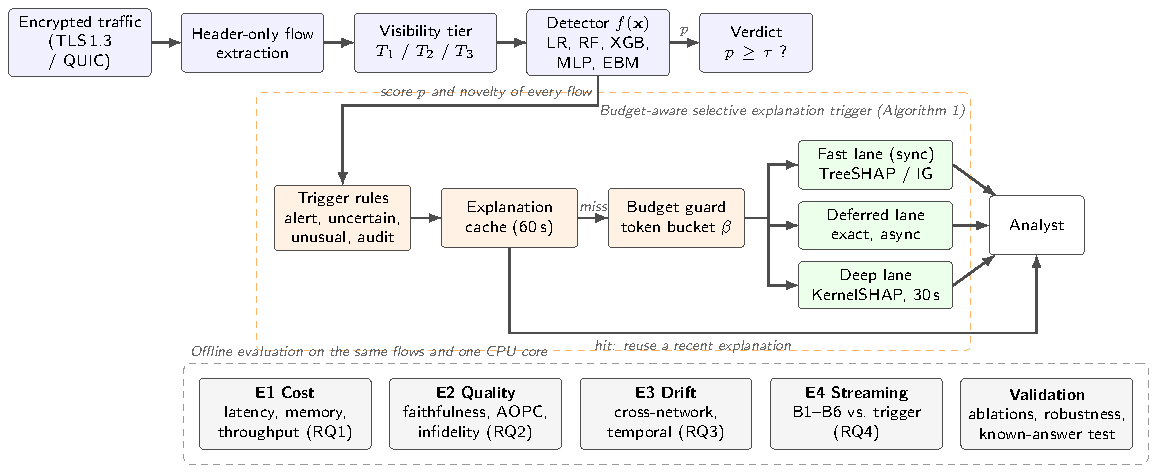
\includegraphics[width=0.86\textwidth]{figures/fig_architecture.pdf}
\caption{Proposed system: online detection with the budget-aware selective explanation trigger (top), and the offline evaluation for RQ1--RQ4 (bottom)}\label{fig:arch}
\end{figure*}

\subsection{Visibility tiers and detectors}
$T_1$ keeps all flow features except identifiers; $T_2$ (TLS~1.3) removes ports and protocol; $T_3$ (QUIC) also removes all TCP-header features, so only sizes, timing, direction and volume remain. Logistic regression (LR), random forest (RF), XGBoost~\cite{chen2016} and a neural network (MLP) are trained on every tier, and the explainable-by-design EBM~\cite{nori2019} on $T_3$. LR, XGBoost and the MLP minimise the class-weighted cross-entropy
\begin{equation}
\mathcal{L}=-\tfrac{1}{n}\textstyle\sum_{i}w_{y_i}\big[y_i\log p_i+(1-y_i)\log(1-p_i)\big],\label{eq:loss}
\end{equation}
where $n$ is the number of training flows, $y_i\in\{0,1\}$ the label, $p_i$ the predicted attack score and $w_y$ a class weight inversely proportional to the class size; RF uses balanced class weights.

\subsection{Explainers and quality metrics}
The explainers are exact TreeSHAP (path and interventional)~\cite{lundberg2020}, KernelSHAP with 100, 500 or 2{,}048 samples~\cite{lundberg2017}, LIME with 500--5{,}000 samples~\cite{ribeiro2016}, Integrated Gradients (IG)~\cite{sundararajan2017}, DeepSHAP~\cite{shrikumar2017}, linear SHAP, the EBM's own contributions and PartitionSHAP (grouped Owen values). \emph{Faithfulness} is the correlation, over random feature subsets $S$, between the attribution mass of $S$ and the score drop when $S$ is replaced by a reference $\bar{\mathbf{x}}$~\cite{bhatt2020}:
\begin{equation}
\mu_F=\mathrm{corr}_{S}\big(\textstyle\sum_{i\in S}\phi_i,\; f(\mathbf{x})-f(\mathbf{x}_{[S\leftarrow\bar{\mathbf{x}}]})\big).\label{eq:faith}
\end{equation}
\emph{Infidelity} is $1-(\mathbf{s}\cdot\mathbf{d})^2/(\|\mathbf{s}\|^2\|\mathbf{d}\|^2)$ over 50 random removals, where $\mathbf{s}$ holds attribution sums and $\mathbf{d}$ score drops~\cite{yeh2019} (0 is best); deletion AOPC~\cite{samek2017} is also reported. Agreement is the overlap of the top-5 features of two explanations (Jaccard, J@5), and drift between networks is $1-\mathrm{J@5}$.

\subsection{Budget-aware trigger}
For every flow, four rules decide whether an explanation is needed: \emph{alert} ($p\ge\tau$); \emph{uncertain} ($|p-\tau|\le\delta$, a band holding 5\% of validation flows); \emph{unusual} (Mahalanobis distance~\cite{ledoit2004} $m(\mathbf{x})\ge\kappa$, the 99th validation percentile); and \emph{audit} (a random share $\alpha=0.5\%$ of benign verdicts). Each request first checks a 60\,s cache of explanations of similar flows. On a miss, a token bucket decides whether a fast exact explanation (TreeSHAP, or IG for the MLP) may run on the detection path: it runs only if the credit covers $\hat{c}_{\mathrm{fast}}$, a running mean of recent fast-explanation times. The bucket holds $b$ seconds of credit, at most $C=50$\,ms, earns $\beta$ times each flow's detection time and pays for all explanation work $c_t$ done for flow $\mathbf{x}_t$ (trigger, cache look-up and explanation):
\begin{equation}
b_{t+1}=\min\big(C,\;b_t+\beta\,t_f(\mathbf{x}_t)\big)-c_t.\label{eq:bucket}
\end{equation}
Without credit, a class-level explanation is shown at once and the exact one is computed on a deferred lane. Strong alerts ($p\ge\tau_{\mathrm{high}}$, set at 0.1\% validation FPR) and uncertain flows also go to a deep lane that runs KernelSHAP-500 and drops jobs that cannot finish within 30\,s. When detection falls more than 100\,ms behind, all work except cache hits pauses. Because work is paid only from credit, the overhead stays bounded:
\begin{equation}
O_{\mathrm{sync}}\le\beta+\frac{C+t_{\max}}{\sum_{\mathbf{x}\in\mathcal{F}}t_f(\mathbf{x})},\label{eq:bound}
\end{equation}
where $t_{\max}$ is the longest fast explanation; the second term is a burst allowance that shrinks as the stream grows. Algorithm~\ref{alg:trigger} summarises the policy.

\begin{algorithm}[!t]
\caption{Budget-aware selective explanation (per flow)}\label{alg:trigger}
\footnotesize
\begin{algorithmic}[1]
\Require flow $\mathbf{x}$, score $p$, thresholds $\tau,\tau_{\mathrm{high}},\delta,\kappa$, audit rate $\alpha$, budget $\beta$, capacity $C$
\State $b\gets\min(C,\,b+\beta\,t_f(\mathbf{x}))$ \Comment{earn credit}
\If{queue delay $>100$\,ms} serve cache hits only; \Return \EndIf
\State $r\gets(p\ge\tau)\lor(|p-\tau|\le\delta)\lor(m(\mathbf{x})\ge\kappa)\lor\mathrm{audit}(\alpha)$
\If{not $r$} \Return verdict only \EndIf
\If{cache holds key$(\mathbf{x})$} \Return cached explanation \EndIf
\If{$b\ge\hat{c}_{\mathrm{fast}}$}
  \State $\boldsymbol{\phi}\gets$ TreeSHAP$(\mathbf{x})$ or IG$(\mathbf{x})$; $b\gets b-c_t$ \Comment{fast lane}
\Else
  \State show class-level explanation; queue $\mathbf{x}$ on deferred lane
\EndIf
\If{$p\ge\tau_{\mathrm{high}}$ or $|p-\tau|\le\delta$}
  \State queue $\mathbf{x}$ on deep lane (KernelSHAP, deadline 30\,s)
\EndIf
\State store the explanation in the cache
\end{algorithmic}
\end{algorithm}

\textbf{Changes after Phase~2.} No feedback was received on Phase~2. Resource limits and problems found while running the system led to these changes: flow records instead of raw packet replay (disk space); an MLP instead of a 1D-CNN (no packet sequences); a repeatable simulated replay instead of \texttt{tcpreplay}; 200 explained flows per setting instead of 1{,}000; a budget that pays for all explanation work; and three of the five planned datasets.

%% ================================================================
\section{Experimental Setup}\label{sec:setup}

\textbf{Datasets.} HIKARI-2021~\cite{hikari} has brute-force, probing and cryptomining attacks over encrypted HTTPS, mixed with benign HTTPS traffic to the same servers. CIC-IDS2017~\cite{cicids2017} (labels corrected by Engelen et al.~\cite{engelen2021}) and CSE-CIC-IDS2018 (corrected by Liu et al.~\cite{liu2022error}) contain the same attack families (reconnaissance, DoS, DDoS, brute force, botnet) on two different networks. After preprocessing, CIC-IDS2017, HIKARI-2021 and CSE-CIC-IDS2018 have 397{,}976, 276{,}211 and 398{,}953 flows, with 50.0\%, 13.3\% and 50.0\% attacks in the test split; $T_1$/$T_2$/$T_3$ keep 84/79/59 features (81/79/60 on HIKARI). To check $T_3$ on real encrypted traffic, the payload was removed from two HIKARI attack captures and flows were extracted with NFStream~\cite{nfstream} before and after: 93--94\% of the bytes disappeared, but all 62 metadata features stayed identical in all 34{,}759 flows, while the TLS server name and fingerprints vanished.

\textbf{Preprocessing.} IP addresses and timestamps are removed, broken values are fixed, and labels are mapped to common attack families. Each dataset is capped at 300k--400k flows without losing small classes and split by time into 60/20/20\% train, validation and test within each attack family. Duplicates and train--test overlaps are removed, and class weights handle imbalance.

\textbf{Baselines.} Detection baselines are the five detectors. Explanation baselines: explain nothing (B1); explain every flow with TreeSHAP or KernelSHAP (B2a/B2b); one global explanation (B3); random flows at the trigger's rate (B4); every alert (B5, as in~\cite{p8}); and a learned FastSHAP-style explainer for every flow (B6)~\cite{fastshap}.

\textbf{Experiments and metrics.} E1 explains the same 200 test flows (100 attack, 100 benign) with every explainer in a fresh process on one pinned core and records latency, throughput and memory. E2 scores the same explanations for faithfulness, infidelity, AOPC and agreement. E3 compares attack-family explanations within and across the two CIC networks. E4 replays 20{,}000 test flows (5\% attacks) at 25\%, 75\% and 150\% of detection capacity, as normal traffic and with an added 3{,}000-flow port-scan flood; all policies see identical traffic. Detection uses precision, recall, F1, false-positive rate (FPR) and ROC-AUC. Comparisons are paired on identical flows (Wilcoxon test with Holm correction~\cite{demsar2006}); equality of explanation quality uses two one-sided tests (TOST, margin 0.05).

\textbf{Implementation.} LR uses L2 regularisation with inverse strength 1; RF 100 trees of depth 20; XGBoost 300 trees of depth 6 (learning rate 0.1); the MLP two hidden layers of 64 and 32 units (Adam, learning rate $10^{-3}$, batch size 1{,}024, 12 epochs); the EBM no interaction terms. Explanations use a 50-point background. The trigger uses $\beta=0.10$, $C=50$\,ms, a 60\,s cache and a 30\,s deep-lane deadline. All runs used an Intel Core i5-1245U laptop (16\,GB RAM, no GPU), Python~3.12.7, scikit-learn~1.9~\cite{pedregosa2011}, XGBoost~3.4, PyTorch~2.15~\cite{paszke2019}, SHAP~0.54, Captum~0.9~\cite{kokhlikyan2020}, InterpretML~0.7.8 and NFStream~6.6.0, with seed 42; timing runs ran alone on an idle machine.

%% ================================================================
\section{Results and Analysis}\label{sec:results}

\subsection{Detection baselines}
Table~\ref{tab:det} shows that hiding ports and TCP headers costs little on CIC-IDS2017: XGBoost moves from F1 0.996 ($T_1$) to 0.981 ($T_3$), RF from 0.992 to 0.988, and only LR loses more (0.896 to 0.867). HIKARI-2021 is much harder: all detectors rank attacks well (ROC-AUC 0.93) but catch only 7--18\% of attacks at 1\% FPR, because its benign traffic includes HTTPS logins to the attacked servers. A threshold tuned for the best validation F1 reaches F1 0.69--0.73 at 11--13\% FPR. Detection takes 0.06--0.08\,ms per flow for LR and the MLP, 0.36--0.55\,ms for the EBM and XGBoost, and 3.5--4.3\,ms for RF.

\begin{table}[!t]
\caption{Detection at 1\% validation FPR. Test FPR on $T_3$: 0.5--0.8\% (CIC), 1.0--2.6\% (HIKARI)}\label{tab:det}
\setlength{\tabcolsep}{1.5pt}
\begin{tabular*}{\columnwidth}{@{\extracolsep\fill}lrrrrrrr@{}}
\toprule
 & \multicolumn{1}{c}{CIC $T_1$} & \multicolumn{3}{c}{CIC-IDS2017 $T_3$} & \multicolumn{3}{c}{HIKARI-2021 $T_3$} \\
\cmidrule(lr){2-2}\cmidrule(lr){3-5}\cmidrule(l){6-8}
Model & F1 & Prec. & Rec. & F1 & Rec. & F1 & ROC \\
\midrule
LR & 0.896 & 0.993 & 0.770 & 0.867 & 0.067 & 0.118 & 0.929 \\
EBM & -- & 0.993 & 0.958 & 0.975 & 0.159 & 0.242 & 0.932 \\
RF & 0.992 & 0.992 & 0.984 & 0.988 & 0.175 & 0.260 & 0.932 \\
XGB & 0.996 & 0.993 & 0.969 & 0.981 & 0.175 & 0.259 & 0.932 \\
MLP & 0.962 & 0.994 & 0.928 & 0.960 & 0.096 & 0.161 & 0.933 \\
\bottomrule
\end{tabular*}
\end{table}

\subsection{RQ1: cost of explanations}
Table~\ref{tab:costfid} shows two cost classes. Model-specific explainers cost about as much as detection: the EBM's contributions take 0.3\,ms, TreeSHAP on XGBoost about 1\,ms and IG 1--3\,ms (RF is the exception: its large trees make TreeSHAP take 10--40\,ms). Model-agnostic explainers take 7--524\,ms, and KernelSHAP grows almost linearly with its sample budget. Memory stays below 176\,MB, and repeated runs differ by only 1.0--13.5\% (e.g.\ KernelSHAP-500 $101.9\pm1.0$\,ms).

With a model-specific explainer, the time per flow grows 1.1--49 times; with a perturbation explainer, 7--1{,}500 times, and 25 of the 44 perturbation settings exceed 100$\times$, so H1 holds only in part. On one core, XGBoost alone handles about 1{,}800 flows/s, 660 with TreeSHAP on every flow and only 9 with KernelSHAP-500. Paying more does not buy quality (Fig.~\ref{fig:pareto}): in 8 of 10 dataset--detector pairs the most faithful explainer is model-specific, usually 22--380 times cheaper than the most faithful perturbation explainer, and cost and faithfulness are not correlated ($\rho_s=-0.19$, $p=0.12$).

\begin{table*}[!t]
\caption{Cost and quality of the explainers on $T_3$ (one CPU core): ms = median time per explanation; Faith.\ = faithfulness (higher is better); Infid.\ = infidelity (lower is better). All 64 settings are in the repository}\label{tab:costfid}
\setlength{\tabcolsep}{3pt}
\begin{minipage}[t]{0.495\textwidth}\centering
\resizebox{\linewidth}{!}{%
\begin{tabular}{@{}llrrrrrr@{}}
\toprule
 & & \multicolumn{3}{c}{CIC-IDS2017} & \multicolumn{3}{c}{HIKARI-2021} \\
\cmidrule(lr){3-5}\cmidrule(l){6-8}
Model & Explainer & ms & Faith. & Infid. & ms & Faith. & Infid. \\
\midrule
LR & LinearSHAP & 0.006 & 0.44 & 0.80 & 0.006 & 0.15 & 0.95 \\
 & LIME-1000 & 23.19 & 0.39 & 0.83 & 22.40 & 0.44 & 0.68 \\
 & KernelSHAP-500 & 44.90 & 0.46 & 0.70 & 43.12 & 0.11 & 0.92 \\
\midrule
EBM & EBM-native & 0.33 & 0.47 & 0.75 & 0.30 & 0.70 & 0.14 \\
 & KernelSHAP-500 & 30.41 & 0.34 & 0.84 & 29.01 & 0.20 & 0.55 \\
\midrule
XGB & TreeSHAP-path & 0.98 & 0.60 & 0.59 & 1.23 & 0.46 & 0.65 \\
 & TreeSHAP-interv & 4.11 & 0.52 & 0.66 & 5.90 & 0.27 & 0.36 \\
 & KernelSHAP-100 & 21.82 & 0.05 & 0.98 & 23.46 & 0.02 & 0.98 \\
 & LIME-1000 & 30.62 & 0.30 & 0.79 & 29.15 & 0.21 & 0.38 \\
 & KernelSHAP-500 & 109.39 & 0.49 & 0.68 & 99.13 & 0.23 & 0.41 \\
 & PartitionSHAP & 174.06 & 0.28 & 0.78 & 176.59 & 0.29 & 0.42 \\
 & KernelSHAP-2048 & 374.10 & 0.50 & 0.67 & 390.83 & 0.30 & 0.47 \\
\bottomrule
\end{tabular}}
\end{minipage}\hfill
\begin{minipage}[t]{0.495\textwidth}\centering
\resizebox{\linewidth}{!}{%
\begin{tabular}{@{}llrrrrrr@{}}
\toprule
 & & \multicolumn{3}{c}{CIC-IDS2017} & \multicolumn{3}{c}{HIKARI-2021} \\
\cmidrule(lr){3-5}\cmidrule(l){6-8}
Model & Explainer & ms & Faith. & Infid. & ms & Faith. & Infid. \\
\midrule
RF & TreeSHAP-path & 9.77 & 0.52 & 0.16 & 39.61 & 0.34 & 0.14 \\
 & TreeSHAP-interv & 13.62 & 0.60 & 0.16 & 37.40 & 0.23 & 0.06 \\
 & LIME-1000 & 35.53 & 0.32 & 0.32 & 34.98 & 0.27 & 0.09 \\
 & KernelSHAP-500 & 114.72 & 0.50 & 0.20 & 127.17 & 0.13 & 0.20 \\
 & KernelSHAP-2048 & 507.81 & 0.57 & 0.15 & 524.30 & 0.18 & 0.09 \\
\midrule
MLP & IG-16 & 1.13 & 0.56 & 0.62 & 1.03 & 0.45 & 0.50 \\
 & DeepSHAP & 1.56 & 0.30 & 0.85 & 1.84 & 0.09 & 0.94 \\
 & KernelSHAP-100 & 7.18 & 0.05 & 0.98 & 6.94 & 0.00 & 0.99 \\
 & LIME-1000 & 23.27 & 0.28 & 0.88 & 22.52 & 0.25 & 0.75 \\
 & KernelSHAP-500 & 24.97 & 0.32 & 0.79 & 23.52 & 0.02 & 0.91 \\
 & KernelSHAP-2048 & 91.94 & 0.31 & 0.77 & 89.76 & 0.04 & 0.92 \\
\bottomrule
\end{tabular}}
\end{minipage}
\end{table*}

\begin{figure*}[!t]
\centering
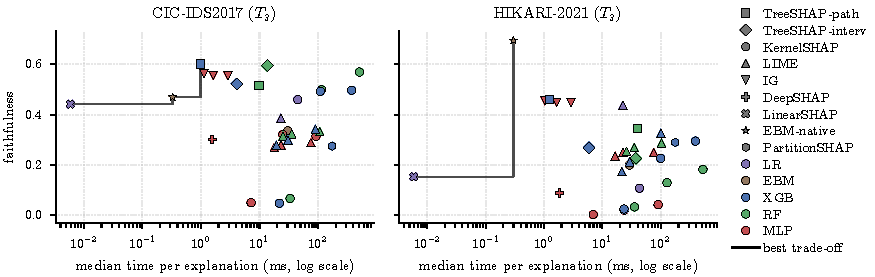
\includegraphics{figures/fig_cost_fidelity_pareto.pdf}
\caption{Cost versus faithfulness of every explainer on $T_3$; the step line is the best trade-off (cheaper and more faithful is better). Fast model-specific explainers form almost the whole frontier}\label{fig:pareto}
\end{figure*}

\subsection{RQ2: fidelity under encryption}
Faithfulness is moderate (mostly 0.2--0.6) and depends strongly on the explainer (Friedman tests, all $p<10^{-36}$). Except for LR, the most faithful explainer of every detector is model-specific: TreeSHAP for XGBoost (0.60 on CIC-IDS2017, 0.46 on HIKARI) and RF (0.60, 0.34), IG for the MLP (0.56, 0.45) and the EBM's own contributions (0.47, 0.70); for LR, a perturbation explainer beats LinearSHAP on both datasets. Infidelity and AOPC rank the explainers in a similar way (Spearman 0.45--0.79 with faithfulness). KernelSHAP with 100 samples is uninformative (faithfulness near 0), while 500 samples are as good as 2{,}048, and DeepSHAP is unreliable for this MLP (0.09--0.30).

H2 expected lower fidelity on $T_3$. Table~\ref{tab:tier} shows the opposite on CIC-IDS2017: faithfulness is significantly higher on $T_3$ for 7 of 8 pairs ($p<0.005$, Holm), e.g.\ KernelSHAP-500 on XGBoost rises from 0.29 to 0.49. On HIKARI the result is mixed (3 pairs worse, 1 better, 4 unchanged). The explanations show why (Table~\ref{tab:tier}, bottom): for DoS flows, \emph{RST Flag Count} carries 25\% of the $T_1$ explanation and the TCP window size another 11\%. These are known recording artefacts of this testbed~\cite{engelen2021}, which encryption hides. On $T_3$ the explanation moves to packet-length statistics, which describe the traffic itself. Explainers also disagree, sharing only about 2 of their top-5 features (J@5 0.19--0.31 for tree models and the MLP), so what an analyst sees depends on the explainer; this agreement does not fall from $T_1$ to $T_3$ (mean 0.23 vs.\ 0.25, 24 pairs).

\begin{table}[!t]
\caption{Top: faithfulness on $T_1$ and $T_3$ for the same flows ($p$: paired Wilcoxon, Holm-corrected). Bottom: qualitative example, TreeSHAP share per feature for the 26 CIC-IDS2017 DoS flows flagged by XGBoost on both tiers}\label{tab:tier}
\setlength{\tabcolsep}{2pt}
\begin{tabular*}{\columnwidth}{@{\extracolsep\fill}llrrrrrr@{}}
\toprule
 & & \multicolumn{3}{c}{CIC-IDS2017} & \multicolumn{3}{c}{HIKARI-2021} \\
\cmidrule(lr){3-5}\cmidrule(l){6-8}
Model & Explainer & $T_1$ & $T_3$ & $p$ & $T_1$ & $T_3$ & $p$ \\
\midrule
XGB & TreeSHAP-path & 0.52 & 0.60 & 3e-05 & 0.49 & 0.46 & 0.69 \\
XGB & TreeSHAP-interv & 0.35 & 0.52 & 1e-14 & 0.35 & 0.27 & 1e-07 \\
XGB & KernelSHAP-500 & 0.29 & 0.49 & 2e-14 & 0.28 & 0.23 & 0.02 \\
XGB & LIME-1000 & 0.23 & 0.30 & 2e-04 & 0.16 & 0.21 & 4e-03 \\
MLP & IG-32 & 0.47 & 0.56 & 3e-07 & 0.49 & 0.45 & 0.69 \\
MLP & DeepSHAP & 0.23 & 0.30 & 7e-04 & 0.10 & 0.09 & 0.69 \\
MLP & KernelSHAP-500 & 0.29 & 0.32 & 0.22 & 0.14 & 0.02 & 9e-13 \\
MLP & LIME-1000 & 0.22 & 0.28 & 4e-03 & 0.27 & 0.25 & 0.69 \\
\bottomrule
\end{tabular*}

\vspace{6pt}
\begin{tabular*}{\columnwidth}{@{\extracolsep\fill}lrlr@{}}
\toprule
\multicolumn{2}{c}{$T_1$ (all features)} & \multicolumn{2}{c}{$T_3$ (QUIC-level)} \\
\cmidrule(r){1-2}\cmidrule(l){3-4}
Feature & Share & Feature & Share \\
\midrule
RST Flag Count & 0.25 & Bwd Pkt Len Std & 0.32 \\
Bwd Pkt Len Std & 0.14 & Bwd Pkt Len Min & 0.07 \\
Bwd Init Win Bytes & 0.11 & Bwd Pkt Len Mean & 0.07 \\
Bwd Pkt Len Min & 0.04 & Bwd IAT Max & 0.04 \\
\bottomrule
\end{tabular*}
\end{table}

\subsection{RQ3: drift across networks}
Fig.~\ref{fig:drift} compares explanations of the four attack families shared by the two CIC networks. Within one network they are stable (J@5 0.99 between random halves of the flows, 0.82 for a model retrained with another seed). Across networks, agreement falls to 0.48 for the same model and to 0.17 when each network has its own model, below both noise levels in 12 of 16 cases. The drift follows the detection loss (Spearman $\rho_s=0.63$, $p=0.008$): for DoS, recall falls from 0.944 to 0.429 and agreement to 0.43, so the transferred model gives confident but outdated reasons for exactly the flows it misses. Transfer costs 20--34 F1 points, and $T_3$ lowers the false-positive rate on the new network (9.9--11.9\% vs.\ 16.8--19.4\%). H3 is supported.

\begin{figure*}[!t]
\centering
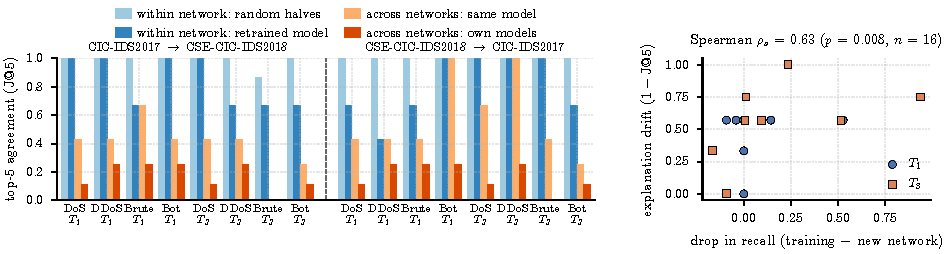
\includegraphics[width=\textwidth]{figures/fig_drift.pdf}
\caption{Left: top-5 agreement of attack-family explanations within one network (two noise levels) and across networks. Right: explanation drift against the drop in recall}\label{fig:drift}
\end{figure*}

\begin{figure*}[!t]
\centering
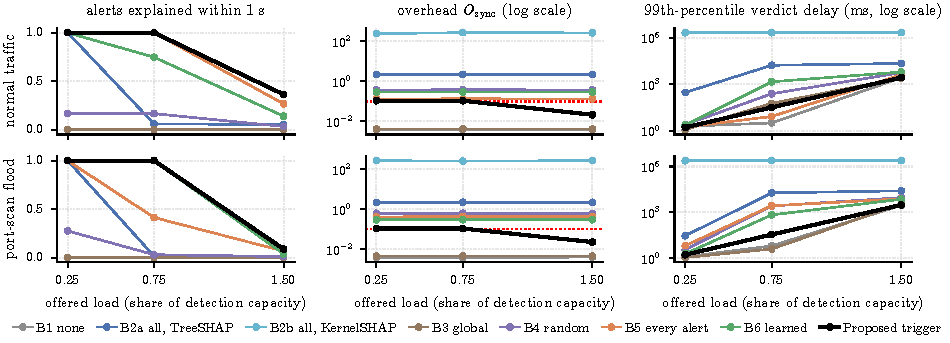
\includegraphics[width=\textwidth]{figures/fig_stream_cic2017_XGB_T3.pdf}
\caption{Explanation policies against load (CIC-IDS2017, XGBoost, $T_3$) for normal traffic (top) and a port-scan flood (bottom); dotted line: budget $\beta=0.10$}\label{fig:stream}
\end{figure*}

\subsection{RQ4: explanation under load}
Table~\ref{tab:stream} and Fig.~\ref{fig:stream} compare the policies on CIC-IDS2017. Explaining every flow is not feasible on one core: even TreeSHAP costs 2.1 times the detection time and delays verdicts by 17--19\,s. In normal traffic, explaining every alert (B5) is affordable; the trigger also explains every alert within 1\,s (overhead 0.106), plus uncertain flows, which include 20 of the 22 attacks the detector misses. During the flood, B5's overhead rises to 0.42 and its delay to 2.7\,s, with only 41\% of alerts explained in time, while the trigger stays at 0.105 and 35\,ms and explains every alert, because the cache answers 61\% of the near-duplicate flood requests. Its explanations are statistically equivalent in quality to fresh ones (TOST, mean difference $-0.008$). At 150\% load no policy keeps up, and the trigger pauses to add no delay. HIKARI shows the same pattern (overhead 0.101--0.102), so H4 holds within detection capacity.

\begin{table}[!t]
\caption{Policies on CIC-IDS2017 at 75\% load. Ovh.\ = $O_{\mathrm{sync}}$; Cov.\ = true alerts explained within 1\,s; Delay = 99th-pct.\ verdict delay (s)}\label{tab:stream}
\setlength{\tabcolsep}{1pt}
\begin{tabular*}{\columnwidth}{@{\extracolsep\fill}lrrrrrr@{}}
\toprule
 & \multicolumn{3}{c}{Normal traffic} & \multicolumn{3}{c}{Port-scan flood} \\
\cmidrule(lr){2-4}\cmidrule(l){5-7}
Policy & Ovh. & Cov. & Delay & Ovh. & Cov. & Delay \\
\midrule
B1 none & 0.00 & 0.00 & 0.003 & 0.00 & 0.00 & 0.006 \\
B2a all, TreeSHAP & 2.14 & 0.06 & 16.7 & 2.15 & 0.01 & 18.7 \\
B2b all, Kernel & 257.7 & 0.00 & 2117 & 242.3 & 0.00 & 2435 \\
B3 global & 0.00 & 0.00 & 0.058 & 0.00 & 0.00 & 0.004 \\
B4 random & 0.37 & 0.16 & 0.243 & 0.60 & 0.03 & 2.58 \\
B5 every alert & 0.13 & 1.00 & 0.008 & 0.42 & 0.41 & 2.68 \\
B6 learned & 0.29 & 0.75 & 1.44 & 0.29 & 1.00 & 0.670 \\
\textbf{Proposed} & \textbf{0.11} & \textbf{1.00} & \textbf{0.032} & \textbf{0.10} & \textbf{1.00} & \textbf{0.035} \\
\bottomrule
\end{tabular*}
\end{table}

%% ================================================================
\section{Base Paper Comparison}\label{sec:compare}

The base papers are the three studies from which the research gap was derived (Table~\ref{tab:base}). Table~\ref{tab:quant} compares this work with them on the closest shared metric, and with related studies whose setups were re-implemented on the same data and laptop~\cite{p2,p5,p6,p9,vitorino2024}.

\begin{table*}[!t]
\caption{Base papers}\label{tab:base}
\setlength{\tabcolsep}{3pt}
\tablebodyfont
\begin{tabularx}{\textwidth}{@{}>{\raggedright\arraybackslash}p{2.05cm}>{\raggedright\arraybackslash}p{1.75cm}YY>{\raggedright\arraybackslash}p{1.6cm}>{\raggedright\arraybackslash}p{1.95cm}Y@{}}
\toprule
Paper & Problem & Method & Dataset & Metrics & Results & Key limitations \\
\midrule
Kalakoti et al.~\cite{kalakoti2026}, 2026 & Explaining a federated IDS & FL-DNN; SHAP and LIME & NSL-KDD, UNSW-NB15, CIC-IoT & F1, faith\-ful\-ness & $>$98\% F1; SHAP more faithful & No cost; offline; unencrypted \\
DMThreat\-Net~\cite{dmthreatnet2026}, 2026 & Early threat detection & Rules + CNN-LSTM ensemble & NSL-KDD, CICIDS\-2017 & F1, FPR, latency & 98.88\% F1; 3.2\,ms & No per-flow XAI; unencrypted \\
Cerasuolo et al.~\cite{cerasuolo2026}, 2026 & Cross-network transfer & RF, XGB, CNNs; Kernel\-SHAP, IG & 8 IoT datasets & Macro-F1, Jaccard & 40--80\% F1 drop & XAI offline; drift not linked to accuracy \\
\bottomrule
\end{tabularx}
\end{table*}

\begin{table*}[!t]
\caption{Numerical comparison. Values marked * come from the original papers; all others were measured in this study. Ranges are compared end to end (lower with lower, upper with upper)}\label{tab:quant}
\setlength{\tabcolsep}{3pt}
\tablebodyfont
\begin{tabularx}{\textwidth}{@{}Ylllll@{}}
\toprule
Comparison (source) & Reference & This study & Absolute & Relative & Note \\
\midrule
\multicolumn{6}{@{}l}{\emph{Base papers: Kalakoti et al.~\cite{kalakoti2026}, DMThreatNet~\cite{dmthreatnet2026}, Cerasuolo et al.~\cite{cerasuolo2026} (other datasets, models or hardware)}} \\
Best SHAP faithfulness~\cite{kalakoti2026} & 0.61--0.79* & 0.46--0.60 & $-$0.15 to $-$0.19 & $-$24 to $-$25\% & TreeSHAP, XGB \\
LIME faithfulness~\cite{kalakoti2026} & 0.20--0.33* & 0.21--0.44 & +0.01 to +0.11 & +5 to +33\% & LIME-1000 \\
Detection F1~\cite{dmthreatnet2026} & 0.9888* & 0.981 & $-$0.008 & $-$0.8\% & NSL-KDD vs.\ CIC \\
Latency per flow~\cite{dmthreatnet2026} & 3.2\,ms* & 1.52\,ms & $-$1.68\,ms & $-$52\% & ours incl.\ XAI \\
Cross-network F1 drop~\cite{cerasuolo2026} & 40--80\%* & 20--35\% & $-$20 to $-$45 pts & $-$50 to $-$56\% & similar networks \\
Agreement of explainers (Jaccard)~\cite{cerasuolo2026} & 0.33--0.93* & 0.19--0.31 & $-$0.14 to $-$0.62 & $-$42 to $-$67\% & top-5, metadata \\
\midrule
\multicolumn{6}{@{}l}{\emph{Related studies, re-implemented on the same data and laptop}} \\
RF macro-F1, 2017$\rightarrow$2018 (P9~\cite{p9}) & 0.208* & 0.222 & +0.014 & +6.8\% & corrected data \\
RF macro-F1, in-domain (P9~\cite{p9}) & 0.989* & 0.808 & $-$0.181 & $-$18.3\% & time vs.\ random split \\
TreeSHAP time per alert (P6~\cite{p6}) & 30--34\,ms* & 0.98\,ms & $-$29 to $-$33\,ms & $-$97\% & explainer reused \\
LIME-5000 time per flow (P5~\cite{p5}) & 4.85--36.38\,s* & 0.090\,s & -- & $-$98.1 to $-$99.8\% & other CPU \\
KernelSHAP time, DNN (P2~\cite{p2}) & 9.2\,s* & 0.092\,s & -- & $-$99\% & flow vs.\ batch \\
Flood overhead (B5, as in~\cite{p8}) & 0.418 & 0.105 & $-$0.313 & $-$74.9\% & same replay \\
Flood 99th-pct.\ delay (B5) & 2.68\,s & 0.035\,s & $-$2.65\,s & $-$98.7\% & same replay \\
Flood alerts explained in 1\,s (B5) & 41.3\% & 100\% & +58.7 points & -- & same replay \\
HIKARI F1 (Vitorino et al.~\cite{vitorino2024}) & 0.835--0.837* & 0.69--0.73 & $-$0.11 to $-$0.15 & -- & leak removed \\
\bottomrule
\end{tabularx}
\end{table*}

\textbf{Methodological comparison.} The base papers explain offline~\cite{kalakoti2026,cerasuolo2026} or not per flow~\cite{dmthreatnet2026}, on plaintext-era features. This work times each explanation with the explainer built once, the cost a streaming IDS pays; uses only metadata checked on packets, so fidelity holds for encrypted traffic; picks the flows to explain under a budget instead of none or all; and uses leak-free time splits and a known-answer test, so scores are not inflated~\cite{arp2022}.

\textbf{Improvement analysis.} The detector nearly matches DMThreatNet's F1 ($-$0.8\%) with encryption-proof features only, and detection plus a TreeSHAP explanation takes 52\% less time than DMThreatNet's detection alone, because TreeSHAP reads the trees instead of querying the model many times. The cross-network drop is about half of Cerasuolo et al.'s, but between more similar networks. The best SHAP faithfulness is about 25\% below Kalakoti et al.'s and explainers agree less than in Cerasuolo et al., because collinear metadata features let explainers pick different but equivalent features. Against the re-implemented studies, per-flow explanation is 97--99.8\% cheaper, mainly because published times include rebuilding the explainer for each alert (30\,ms, against 0.98\,ms per explanation) or are batch averages; during the flood the trigger cuts overhead by 74.9\% and delay by 98.7\% against explaining every alert, because the cache absorbs near-duplicate flows and the budget defers work. On P9's cross-dataset test the result is slightly better (+0.014 macro-F1), even without ports and TCP headers (0.217).

\textbf{Fairness and limitations.} Some results are lower. The in-domain macro-F1 is below P9's (0.808 vs.\ 0.989) because the time split keeps near-copies of the same attack session out of training, which a random split does not~\cite{arp2022}. The published 83\% F1 on HIKARI-2021~\cite{vitorino2024} could not be reproduced: the public file is sorted by traffic type and contains two row-number columns, one of which alone separates attacks from benign flows (ROC-AUC 0.93); this work removes both. Hardware and the timed unit (instance, alert, batch) also differ between studies, and the base-paper values come from other datasets and models (NSL-KDD, IoT networks, a federated DNN), so these rows show where this work stands, not exact gains.

%% ================================================================
\section{Ablation Study}\label{sec:ablation}

\textbf{Trigger components.} Table~\ref{tab:abl} removes or changes one part of the trigger at a time on the same replay. Without the uncertainty rule (A1), more alerts are explained instantly (86\% instead of 57\%), but none of the 20 missed attacks is explained; it is the only part that shows analysts the detector's mistakes. The novelty rule (A2) costs the most and only pays off when the network changes. Without the cache (A3), instant coverage falls to 5--15\%; without the budget limit (A4), overhead doubles and the delay triples; KernelSHAP on the detection path (A5b) explains no alert in time; and without the deep lane (A5a), delay falls slightly but strong and uncertain alerts get no KernelSHAP explanation. Overhead follows the budget down to about 0.05, the trigger's own cost (A6).

\begin{table}[!t]
\caption{Trigger ablations (CIC-IDS2017, 75\% load). Inst.\ = alerts explained on the detection path; Delay in ms}\label{tab:abl}
\setlength{\tabcolsep}{1pt}
\begin{tabular*}{\columnwidth}{@{\extracolsep\fill}lrrrrrr@{}}
\toprule
 & \multicolumn{3}{c}{Normal traffic} & \multicolumn{3}{c}{Port-scan flood} \\
\cmidrule(lr){2-4}\cmidrule(l){5-7}
Variant & Ovh. & Inst. & Delay & Ovh. & Inst. & Delay \\
\midrule
\textbf{Full trigger} & 0.11 & 0.57 & 32 & 0.10 & 0.88 & 35 \\
A1 no uncertainty & 0.11 & 0.86 & 12 & 0.10 & 0.96 & 58 \\
A2 no novelty & 0.11 & 0.73 & 36 & 0.09 & 0.92 & 151 \\
A3 no cache & 0.11 & 0.15 & 38 & 0.11 & 0.05 & 18 \\
A4 no budget limit & 0.24 & 1.00 & 100 & 0.23 & 1.00 & 113 \\
A5a no deep lane & 0.11 & 0.60 & 18 & 0.10 & 0.85 & 23 \\
A5b KernelSHAP only & 0.05 & 0.00 & 12 & 0.06 & 0.00 & 6 \\
A6 budget 5\% & 0.06 & 0.21 & 12 & 0.06 & 0.31 & 26 \\
A6 budget 20\% & 0.20 & 0.91 & 108 & 0.20 & 0.98 & 31 \\
\bottomrule
\end{tabular*}
\end{table}

\textbf{Features and explainer.} On HIKARI, timing features alone (A8) detect nearly as well as all features (F1 0.248 vs.\ 0.262) but give explanations with near-zero faithfulness (0.06), so good detection does not guarantee a good explanation. Grouped Owen attributions (A10) are less faithful than KernelSHAP on CIC-IDS2017 (0.30 vs.\ 0.49) and 1.7$\times$ slower, and a 10-point KernelSHAP background (A11) loses a third of the faithfulness.

\textbf{Known-answer test.} A random feature was added to the CIC-IDS2017 $T_3$ data and benign flows with high values of it were relabelled as attacks, so it is the true reason for those alerts and irrelevant for real ones (Table~\ref{tab:sanity}). TreeSHAP, KernelSHAP-500 and PartitionSHAP always rank it first for planted attacks and almost never for real ones; LIME finds it but also blames it for 88\% (XGBoost) and 55\% (MLP) of real attacks, and DeepSHAP never finds it, as in RQ2.

\begin{table}[!t]
\caption{Known-answer test: share of planted attacks (Found, ideal 1) and real attacks (Wrong, ideal 0) where the planted feature ranks first}\label{tab:sanity}
\setlength{\tabcolsep}{2pt}
\begin{tabular*}{\columnwidth}{@{\extracolsep\fill}llrr@{}}
\toprule
Model & Explainer & Found & Wrong \\
\midrule
XGB & TreeSHAP (both) & 1.00 & 0.00--0.01 \\
XGB & KernelSHAP-500 & 1.00 & 0.00 \\
XGB & PartitionSHAP & 1.00 & 0.00 \\
XGB & KernelSHAP-100 & 0.85 & 0.02 \\
XGB & LIME-1000 & 1.00 & 0.88 \\
MLP & IG-16 & 0.99 & 0.16 \\
MLP & KernelSHAP-500 & 1.00 & 0.05 \\
MLP & LIME-1000 & 1.00 & 0.55 \\
MLP & DeepSHAP & 0.00 & 0.00 \\
\bottomrule
\end{tabular*}
\end{table}

\textbf{Robustness.} Up to 50\% timing jitter or size padding leaves CIC-IDS2017 XGBoost at F1 0.981--0.984 with similar top-5 explanations (J@5 0.85--0.91), but 5\% padding cuts the HIKARI F1 from 0.262 to 0.078.

%% ================================================================
\section{Discussion}\label{sec:discussion}

\textbf{Why it works.} Model-specific explainers read the model's structure (trees, gradients, additive terms) and cost about one model call, while perturbation explainers need hundreds; hence cost depends on the explainer--detector pair. Encryption-proof metadata removes threshold-like artefacts (flags, ports, window sizes) that additive explanations describe poorly, so fidelity rose on CIC-IDS2017. The trigger works because costly cases repeat (cache hits) or can wait.

\textbf{Strengths and practical implications.} Cost and fidelity are measured on the same flows and core, the tiers are checked on real packets, the explainers face a known-answer test, and the overhead has a proven bound (Eq.~\ref{eq:bound}). XGBoost with TreeSHAP, or an EBM, detects and explains a flow for 1.8--4.2 times the cost of detection alone with the best measured fidelity, so detector and explainer should be chosen together, with KernelSHAP and LIME on a background lane. As explainers disagree, a team should fix one and check its fidelity on its own traffic; drift can then flag a network change before labels arrive.

\textbf{Limitations, failure cases and threats to validity.} QUIC visibility is imitated by removing columns, not measured on real QUIC traffic, and the only truly encrypted dataset (HIKARI) has weak detectors. DeepSHAP fails on the MLP, LIME blames irrelevant features, the deep lane (about 9 KernelSHAP explanations/s) serves only 24--26\% of escalations within 30\,s, and the HIKARI detector is fragile to padding. \emph{Internal validity:} one laptop, 200 flows per setting and one training seed, with isolated, repeated timing runs. \emph{Construct validity:} faithfulness depends on the removal reference, but the known-answer test gives the same ranking. \emph{External validity:} two CIC networks and one encrypted dataset. \emph{Conclusion validity:} all $p$-values are Holm-corrected.

\textbf{Research gap and objectives.} H1 is partly supported (25 of 44 settings), H2 is rejected on CIC-IDS2017 and mixed on HIKARI, and H3 and H4 hold (H4 within capacity). All gaps of Section~\ref{sec:intro} are closed: cost is timed per flow (G1, Phase~1), fidelity on encryption-proof features (G2), drift tracks accuracy loss (G3), and a budget-aware policy picks flows to explain (G4, Phase~2).

%% ================================================================
\section{Conclusion and Future Work}\label{sec:conclusion}

This paper measured the cost and fidelity of nine explainers on five detectors for encrypted-traffic IDS and proposed a budget-aware selective trigger. Model-specific explainers were usually the cheapest and most faithful, hiding transport headers removed artefacts rather than explainability, drift followed accuracy loss across networks, and the trigger explained every alert within 1\,s at about 10\% overhead, even during a flood. Future work will use real QUIC and DNS-over-HTTPS traffic, packet-sequence detectors, edge devices, an online budget and analyst studies.

\backmatter

\section*{Declarations}

\bmhead{Funding} No funding was received.

\bmhead{Conflict of interest} None.

\bmhead{Ethics approval} Not applicable.

\bmhead{Data and code availability} HIKARI-2021 is on Zenodo (record 6463389); the corrected CIC-IDS2017 and CSE-CIC-IDS2018 releases are from their authors~\cite{engelen2021,liu2022error}. Code, results, figures and a demo notebook (MIT License): \url{https://github.com/ahmed-raza19/xai-encrypted-ids}.

\bmhead{AI-tool usage} The authors used an AI assistant (Claude, Anthropic) to help write and debug the experiment code, run the analysis scripts, and draft and edit the text. All experiments were run on the authors' machine with the code in the repository, and the authors reviewed the results and take full responsibility for the content.

\bibliography{references}

\end{document}
